\section{ResNet training reproducibility and continuation checks}
\label{app:resnet_checks}

\subsection{Independent training seeds}

We repeat the original 50-epoch ResNet training using two additional random seeds, changing the initialization and stochastic training sequence while keeping the training and validation objects, architecture, normalization, batch size, augmentation rule, loss, and optimization schedule fixed.
Each run completes 111\,350 updates, and its checkpoint is selected using the same full-field validation mean absolute error as the original run.
Table~\ref{tab:resnet_seeds} reports both the selected and final checkpoints; the source-specific errors do not determine this selection.
The original seed remains the main comparison model, rather than selecting among seeds using these diagnostics.

\begin{table*}[t]
    \centering
    \caption{Validation errors for independent ResNet training seeds.}
    \label{tab:resnet_seeds}
    \begin{tabular}{llrrrr}
        \hline\hline
        Seed & Checkpoint & Epoch & Source MAE & Source RMSE & Outside-source RMSE \\
        \hline
        20261016 & Selected & 49 & 0.0203059 & 0.0601735 & 0.0139575 \\
        20261018 & Selected & 46 & 0.0202803 & 0.0601034 & 0.0139342 \\
        20261019 & Selected & 48 & 0.0203096 & 0.0600667 & 0.0139416 \\
        \hline
        20261016 & Final & 50 & 0.0203161 & 0.0602433 & 0.0139571 \\
        20261018 & Final & 50 & 0.0202607 & 0.0598323 & 0.0139410 \\
        20261019 & Final & 50 & 0.0203063 & 0.0600158 & 0.0139413 \\
        \hline
    \end{tabular}
    \tablefoot{Errors are in MJy\,sr$^{-1}$, measured over the fixed regions of all 2118 validation objects.
    Each regional metric is computed per object before averaging with equal weights.
    Selected checkpoints minimize the original full-field validation MAE, so they need not minimize a regional metric in this table.}
\end{table*}

\begin{figure*}[t]
    \centering
    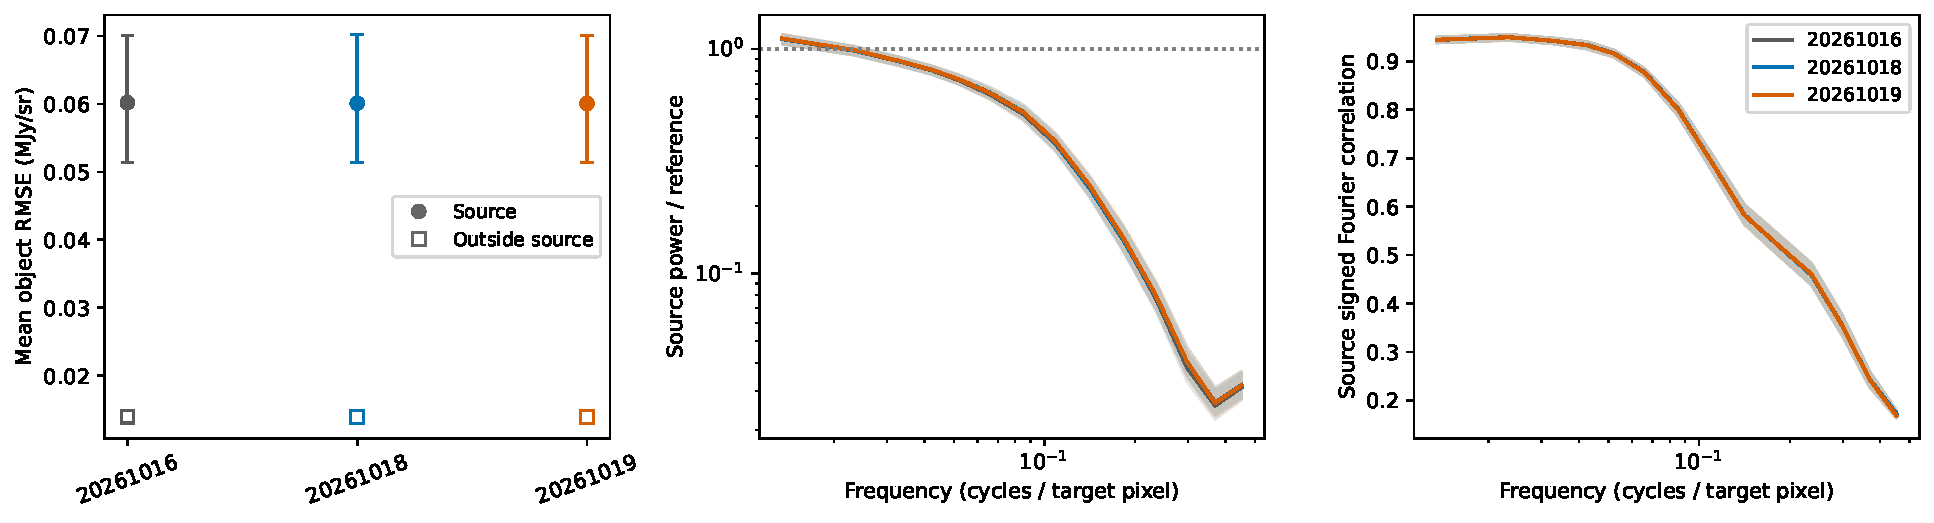
\includegraphics[width=\textwidth]{figs/resnet_seed_comparison_v01.pdf}
    \caption{Independent-seed reproducibility of the original ResNet training recipe, using each run's validation-selected checkpoint.
    Left: source (filled circles) and outside-source (open squares) mean per-object RMSE for all 2118 validation objects.
    Middle and right: source-only power ratios and signed Fourier correlations on the same 1363 completely valid cutouts used in Fig.~\ref{fig:pixel_comp}.
    Windows and spectral definitions follow Sect.~\ref{sc:regional_structure}; the horizontal axis here is frequency in cycles per target pixel.
    Whiskers and shaded bands are conditional 95\% spatial-block intervals for each trained model, not uncertainty across training seeds.
    Differences between the three markers or curves describe the observed seed variation.}
    \label{fig:resnet_seeds}
\end{figure*}

Across the three selected checkpoints, the mean and sample standard deviation of source RMSE are $0.0601145$ and $0.0000542$ MJy\,sr$^{-1}$; outside-source values are $0.0139444$ and $0.0000119$ MJy\,sr$^{-1}$.
These are descriptive statistics over three training runs, distinct from the conditional spatial-block intervals plotted for each run.
In the 6--15 target-pixel spectral band, source power ratios span 0.417--0.425 and signed correlations span 0.7374--0.7382.
The narrow ranges support the stability of the measured ResNet behaviour under these seed changes.

\subsection{Matched continuation experiments}

Both continuations start from the same original epoch-49 checkpoint, preserving its Adam state and using identical batches and paired augmentations.
Each receives ten extra epochs, or 22\,270 updates, with a new per-update cosine learning-rate schedule from $10^{-5}$ to $10^{-6}$.
The control retains the original valid-pixel mean absolute error.
The alternative averages source and outside-source mean absolute errors with weights 0.5 and 0.5 within each object, then averages objects equally.
Training masks use the same detection prescription as Sect.~\ref{sc:regional_structure} on the full $205\times205$ target field; both regions are nonempty for every training object.
For both branches, the lowest mean source MAE on the fixed central validation region selects the checkpoint, with the unchanged parent included as an epoch-zero candidate.
This common continuation criterion differs from the full-field MAE used to select the original training checkpoints.

\begin{table*}[t]
    \centering
    \caption{Validation errors for matched ResNet continuations from one parent checkpoint.}
    \label{tab:resnet_continuations}
    \begin{tabular}{lrrrr}
        \hline\hline
        Variant & Extra epochs & Source MAE & Source RMSE & Outside-source RMSE \\
        \hline
        Original checkpoint & 0 & 0.0203059 & 0.0601735 & 0.0139575 \\
        Original-loss control, selected & 5 & 0.0202381 & 0.0594465 & 0.0139444 \\
        Equal-region loss, selected & 5 & 0.0198781 & 0.0588579 & 0.0142922 \\
        Original-loss control, final & 10 & 0.0202892 & 0.0600835 & 0.0139518 \\
        Equal-region loss, final & 10 & 0.0199232 & 0.0594867 & 0.0142954 \\
        \hline
    \end{tabular}
    \tablefoot{Units and regional aggregation match Table~\ref{tab:resnet_seeds}.
    Both branches complete ten extra epochs; selected rows minimize source MAE among epochs zero through ten.
    The two branches share one parent and are not independent training-seed repetitions.}
\end{table*}

The equal-region loss produces a source/outside-source trade-off (Table~\ref{tab:resnet_continuations}).
Its selected checkpoint improves source MAE by 2.11\% and source RMSE by 2.19\% relative to the parent, while worsening outside-source RMSE by 2.40\%.
At 3--6 target-pixel wavelengths, the change in signed source correlation is $+0.00057$, with paired 95\% spatial-block interval $[-0.00063,+0.00167]$.
The original-loss control gives $+0.00248$ with interval $[+0.00080,+0.00410]$ in this band.
Additional power retention therefore does not imply a clear gain in fine-scale reference alignment.

Shape comparisons retain the same successful objects across the reference, the parent, and both selected and final continuations: 1628 objects for fixed moments and 1677 for adaptive moments.
For the selected equal-region continuation minus the parent, the ellipticity component RMSE changes by $+0.00031$ with interval $[-0.00294,+0.00331]$ for fixed moments and by $-0.00074$ with interval $[-0.00458,+0.00274]$ for adaptive moments.
Neither interval establishes an improvement.
Across all attempted objects, fixed-moment successes increase from 1786 to 1845, whereas adaptive-moment successes decrease from 1742 to 1723; the success population is therefore reported separately from the conditional error comparison.
These are observed-shape diagnostics, not PSF-corrected or calibrated shear measurements.

All continuation intervals use 2000 paired spatial-block resamples with equal object weights.
They condition on this parent, field, and validation-based selection, and do not account for variation between training seeds or checkpoint selection.
The final-epoch rows show that some selected-epoch gains diminish with further updates.
Together with the independent-seed check, these results support retaining the original ResNet for the main comparison while recording the continuation trade-off separately.
